\section{Verkauf}
\autorbeginn{Marcel}
\label{sec:ui-verkauf}

Der Verkaufsbildschirm gibt dem Spieler die Möglichkeit seine produzierten Raumschiffe am Absatzmarkt anzubieten.
 
Der Bildschirm enthält die drei verschiedenen Raumschifftypen. Neben jedem Raumschiff wird dem Spieler die verfügbare Menge, das heißt die in der letzten Periode produzierten oder die im Lager verfügbaren fertigen Raumschiffe, angezeigt. Unterhalb der verfügbaren Menge, werden die gesamten Herstellungskosten des Raumschifftyps dargestellt. 
 
Aus dem Verkaufspreis, den der Spieler in einem gelb hinterlegten Textfeld eingeben kann und den gesamten Herstellungskosten ergibt sich ein Deckungsbeitrag, den der jeweilige Raumschifftyp zum Unternehmenserfolg beiträgt. Dieser Deckungsbeitrag wird zwischen den Herstellungskosten und dem festgelegten Verkaufspreis angezeigt.
 
Hat der Spieler für jeden Raumschifftyp einen Preis festgelegt, so wird ihm der gesamte Verkaufspreis in einem grün hinterlegten Textfeld angezeigt. Über den Button unterhalb des gesamten Verkaufspreises kann der Spieler seine Preisangebote abgeben und somit die produzierten Raumschiffe am Absatzmarkt anbieten.  Nachfolgend wird der Verkaufsbildschirm dargestellt (s. \ref{img:ui-verkauf}).

\begin{figure}[h]
  \centering
  \fbox{
    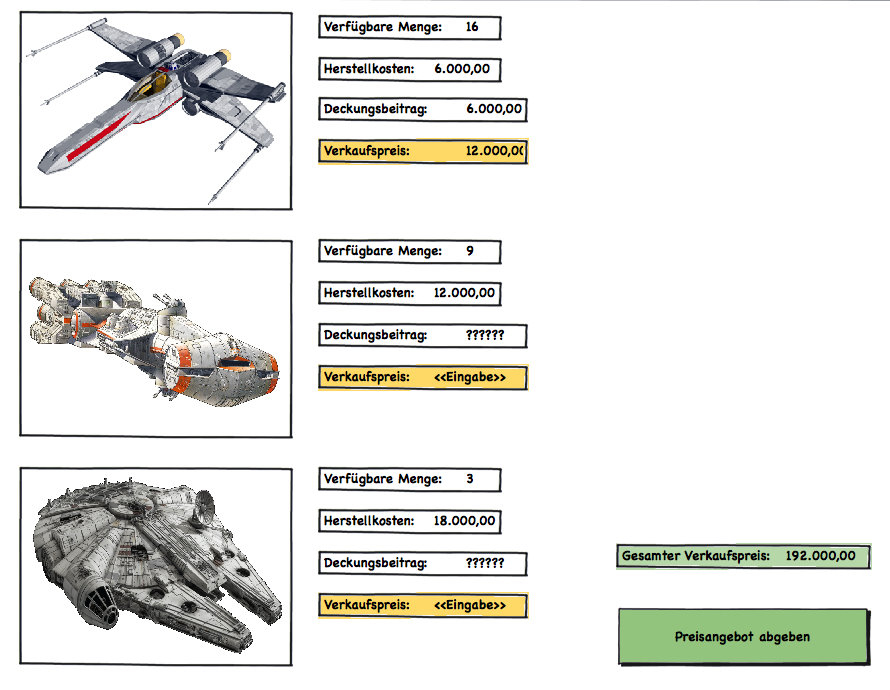
\includegraphics[width=0.9\textwidth]{40_UI/70_Verkauf/Verkauf.jpg}
  }
  \caption{Verkauf}
  \label{img:ui-verkauf}
\end{figure}

\autorende{}